\documentclass[10pt]{article}
\usepackage[letterpaper,portrait,margin=0.34in]{geometry}
\usepackage[T1]{fontenc}
\usepackage[utf8]{inputenc}
\usepackage{lmodern}
\usepackage{microtype}
\usepackage{amssymb}
\usepackage{xcolor}
\usepackage{graphicx}
\usepackage{tabularx,booktabs,array}
\usepackage{enumitem}
\usepackage{tikz}
\usetikzlibrary{arrows.meta,calc}
\usepackage[hidelinks]{hyperref}

% Same palette and spacing as the Deliverable 2 page.
\definecolor{navy}{HTML}{12324A}
\definecolor{blue}{HTML}{1F6E8C}
\definecolor{ice}{HTML}{EAF3F6}
\definecolor{ink}{HTML}{17232B}
\definecolor{muted}{HTML}{52616B}
\definecolor{alert}{HTML}{A3382F}
\definecolor{code}{HTML}{F3EEE6}
\definecolor{codeline}{HTML}{9C7A4A}
\newcommand{\repo}{https://github.com/benjaminnalvear-dev/genai-vio-meeting-minutes}
\newcommand{\video}{\textit{video: link pending}}

\pagestyle{empty}
\setlength{\parindent}{0pt}
\setlength{\parskip}{0.8pt}
\setlist[itemize]{leftmargin=0.9em,itemsep=0.1pt plus 1.5pt,topsep=0.2pt plus 1pt,parsep=0pt}
\renewcommand{\arraystretch}{1.0}
\setlength{\tabcolsep}{2.4pt}
\color{ink}
\newcommand{\firstsectionbar}[1]{{\bfseries\sffamily\color{navy}#1}\par\vspace{1.4pt}}
\newcommand{\sectionbar}[1]{\vspace{3.6pt plus 1fill}{\bfseries\sffamily\color{navy}#1}\par\vspace{1.4pt}}
\newcommand{\tabfont}{\fontsize{7.1}{7.85}\selectfont}
\newcolumntype{Y}{>{\raggedright\arraybackslash}X}

\begin{document}
\sffamily
\fontsize{8.05}{8.95}\selectfont

{\fontsize{13.2}{14.5}\selectfont\bfseries Verifiable meeting minutes with three agents that decide}\hfill
{\normalsize\bfseries Deliverable 3}\par
\vspace{0.5pt}
{\fontsize{7.2}{7.8}\selectfont Benjamin Alvear \textbullet{} Xavier Godoy \textbullet{} Eduardo Ruiz \textbullet{} Damian Vera
\hfill Generative Artificial Intelligence (580694) \textbullet{} 31-oct-2026 \textbullet{} \href{\repo}{repository on GitHub} \textbullet{} \video}

% ---------------------------------------------------------------- agent graph
\vspace{2pt}
{\color{blue}\rule{\linewidth}{0.7pt}}\par
\vspace{8pt}
\noindent\resizebox{\linewidth}{!}{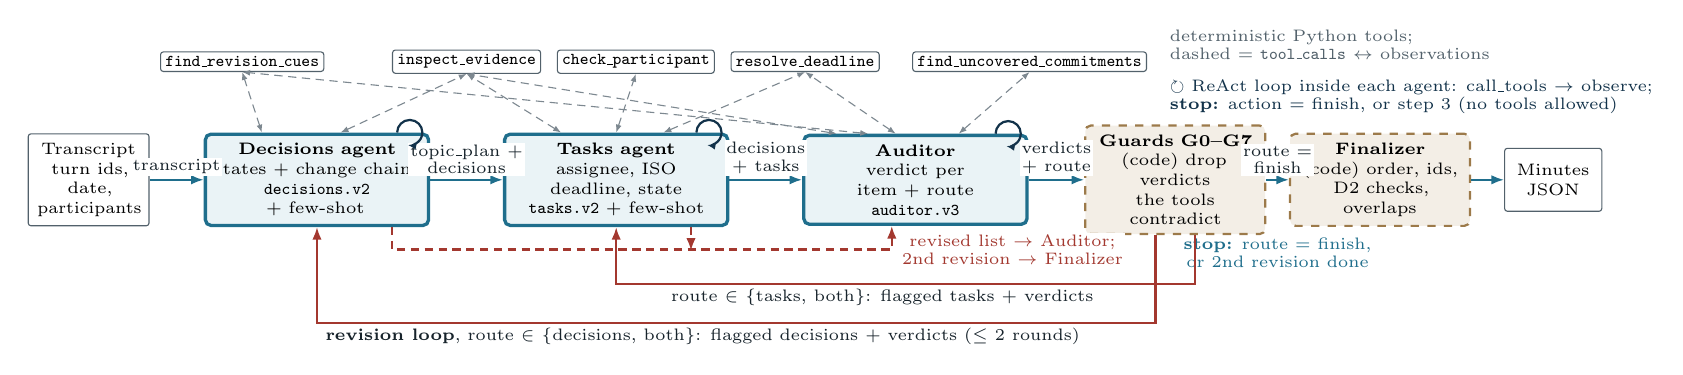
\begin{tikzpicture}[
  font=\fontsize{6.5}{7.1}\selectfont,
  agent/.style={draw=blue,very thick,rounded corners=2pt,fill=ice,align=center,minimum height=10.5mm,text width=2.6cm},
  code/.style={draw=codeline,dashed,thick,rounded corners=2pt,fill=code,align=center,minimum height=10.5mm,text width=2.05cm},
  io/.style={draw=muted,rounded corners=1pt,align=center,minimum height=8mm,text width=1.3cm},
  tl/.style={draw=muted,fill=white,rounded corners=1pt,align=center,inner sep=1.7pt,font=\ttfamily\fontsize{6.1}{6.5}\selectfont},
  flow/.style={-{Latex[length=1.6mm]},thick,color=blue},
  back/.style={-{Latex[length=1.6mm]},thick,color=alert},
  use/.style={{Latex[length=1.0mm]}-{Latex[length=1.0mm]},densely dashed,thin,color=muted!75},
  lbl/.style={font=\fontsize{6.0}{6.5}\selectfont,text=ink,align=center,fill=white,inner sep=0.7pt},
]
\node[io] (tr) at (0.65,0) {Transcript\\turn ids, date,\\participants};
\node[agent] (dec) at (3.55,0) {\textbf{Decisions agent}\\states + change chains\\\texttt{decisions.v2} + few-shot};
\node[agent] (tsk) at (7.35,0) {\textbf{Tasks agent}\\assignee, ISO deadline, state\\\texttt{tasks.v2} + few-shot};
\node[agent] (aud) at (11.15,0) {\textbf{Auditor}\\verdict per item + route\\\texttt{auditor.v3}};
\node[code] (grd) at (14.45,0) {\textbf{Guards G0--G7}\\(code) drop verdicts\\the tools contradict};
\node[code] (fin) at (17.05,0) {\textbf{Finalizer}\\(code) order, ids,\\D2 checks, overlaps};
\node[io,text width=1.0cm] (out) at (19.25,0) {Minutes\\JSON};

% handoffs
\draw[flow] (tr) -- node[lbl,above=1pt]{transcript} (dec);
\draw[flow] (dec) -- node[lbl,above=1pt]{topic\_plan +\\decisions} (tsk);
\draw[flow] (tsk) -- node[lbl,above=1pt]{decisions\\+ tasks} (aud);
\draw[flow] (aud) -- node[lbl,above=1pt]{verdicts\\+ route} (grd);
\draw[flow] (grd) -- node[lbl,above=1pt]{route =\\finish} (fin);
\draw[flow] (fin) -- (out);
\node[lbl,text=blue,anchor=north] at ($(grd.south east)!0.5!(fin.south west)+(0,-0.06)$) {\textbf{stop:} route = finish,\\or 2nd revision done};

% revision loop (below)
\draw[back] ($(grd.south)+(0.25,0)$) -- ++(0,-0.62) -| node[lbl,pos=0.27,below=0.6pt]{route $\in$ \{tasks, both\}: flagged tasks + verdicts} (tsk.south);
\draw[back] ($(grd.south)+(-0.25,0)$) -- ++(0,-1.12) -| node[lbl,pos=0.27,below=0.6pt]{\textbf{revision loop}, route $\in$ \{decisions, both\}: flagged decisions + verdicts ($\le$ 2 rounds)} (dec.south);
% return handoff after a revision
\draw[back,densely dashed] ($(dec.south)+(0.95,0)$) |- ($(aud.south)+(-0.3,-0.3)$) -- ($(aud.south)+(-0.3,0)$);
\draw[back,densely dashed] ($(tsk.south)+(0.95,0)$) -- ($(tsk.south)+(0.95,-0.3)$);
\node[lbl,text=alert,anchor=north west] at ($(aud.south)+(-0.2,-0.08)$) {revised list $\to$ Auditor;\\2nd revision $\to$ Finalizer};

% ReAct self-loops on each agent
\foreach \a in {dec,tsk,aud}{
  \draw[-{Latex[length=1.1mm]},thick,color=navy] ($(\a.north east)+(-0.42,0)$) arc[start angle=180,end angle=-100,radius=0.16];
}

% tools (above)
\node[tl] (frc) at (2.6,1.5) {find\_revision\_cues};
\node[tl] (ie)  at (5.45,1.5) {inspect\_evidence};
\node[tl] (cp)  at (7.6,1.5) {check\_participant};
\node[tl] (rd)  at (9.75,1.5) {resolve\_deadline};
\node[tl] (fuc) at (12.6,1.5) {find\_uncovered\_commitments};
\draw[use] ($(dec.north)+(-0.7,0)$) -- (frc.south);
\draw[use] ($(dec.north)+(0.3,0)$) -- (ie.south);
\draw[use] ($(tsk.north)+(-0.7,0)$) -- (ie.south);
\draw[use] ($(tsk.north)+(0.0,0)$) -- (cp.south);
\draw[use] ($(tsk.north)+(0.6,0)$) -- (rd.south);
\draw[use] ($(aud.north)+(-1.0,0)$) -- (ie.south);
\draw[use] ($(aud.north)+(-0.6,0)$) -- (frc.south);
\draw[use] ($(aud.north)+(-0.25,0)$) -- (rd.south);
\draw[use] ($(aud.north)+(0.55,0)$) -- (fuc.south);
\node[lbl,text=muted,anchor=west,align=left] at (14.35,1.72) {deterministic Python tools;\\dashed = \texttt{tool\_calls} $\leftrightarrow$ observations};
\node[lbl,text=navy,anchor=west,align=left] at (14.35,1.05) {$\circlearrowright$ ReAct loop inside each agent: call\_tools $\to$ observe;\\\textbf{stop:} action = finish, or step 3 (no tools allowed)};
\end{tikzpicture}}
\par\vspace{7pt}
% Both columns stretch to this height (largest that keeps one page); section gaps absorb the slack.
\newlength{\colheight}\setlength{\colheight}{8.0in}

% ---------------------------------------------------------------- left column
\begin{minipage}[t][\colheight][s]{0.492\textwidth}
\vspace{0pt}
\firstsectionbar{1. PROBLEM AND WHY THE BENCHMARK IS HARD}
A Spanish meeting transcript becomes JSON minutes: each \textbf{decision} has a state (\texttt{final}, \texttt{superseded}, \texttt{rejected}, \texttt{pending}) and points to the decision it replaces; each \textbf{task} has an assignee, an ISO deadline and a condition; every item cites its evidence turn. D2 (Ministral~3B, constrained JSON + deterministic tools, two fixed passes) left four errors (D2 report, same 10 test meetings): \textbf{E1} non-final decision states (10/30 found); \textbf{E2} relative deadlines (12/39 right); \textbf{E3} confirmed tasks emitted as \texttt{pending} (47/56); \textbf{E4} nothing checks that the cited turn supports the item.

\smallskip
{\tabfont
\begin{tabularx}{\linewidth}{@{}lrY@{}}
\toprule
Test set: M01--M10, natural dialogue, 347 turns & n & Why it is hard \\
\midrule
Decisions & 56 & only 26 are a plain \texttt{final}: 11 superseded, 11 rejected, 8 pending \\
Topics revised during the meeting & 20 & chains of up to 3 proposals \\
Conditional decisions / tasks & 10 / 15 & keep the condition, do not drop the item \\
Tasks & 53 & 29 relative deadlines, 8 with a time, 22 must stay \texttt{null} \\
Mentions of absent people & 24 & they cannot be assignees \\
\bottomrule
\end{tabularx}}

\sectionbar{2. AGENT DESIGN}
{\tabfont
\begin{tabularx}{\linewidth}{@{}l Y Y@{}}
\toprule
Agent & Receives $\to$ returns & Decides; stops \\
\midrule
Decisions & transcript (+ flagged items) $\to$ \texttt{topic\_plan}, decisions & call tools or finish, per step; stops at \texttt{finish} or step 3 \\
Tasks & transcript + decisions $\to$ tasks & same ReAct loop, own tools \\
Auditor & transcript + both lists $\to$ verdicts, route & \texttt{finish}, \texttt{decisions}, \texttt{tasks} or \texttt{both}; $\le$2 rounds \\
\bottomrule
\end{tabularx}}
\smallskip

\textbf{Why this split.} Decisions and tasks fail differently (E1 vs E2/E3) and need different tools, so each specialist gets a short, focused prompt, which matters for a 3B model. Only the Auditor sees the whole minutes, so it covers E4 and omissions across lists. Guards and Finalizer are code and never call the model. \textbf{The agents do decide:} on test they made 212 tool calls; 3 meetings closed after the first audit and 7 ran two revision rounds; the guards rejected 41 of the Auditor's 70 flags (e.g.\ a \texttt{wrong\_state} on a turn that literally says ``pendiente'') and 20 duplicate items.

\sectionbar{3. PROMPTING TECHNIQUES (THE PROMPT REPORT TAXONOMY)}
{\tabfont
\begin{tabularx}{\linewidth}{@{}Y l l r r@{}}
\toprule
Technique (category) & Where & Fixes & $\Delta$F1 dec. & tasks \\
\midrule
ReAct tool use (Agents) & all & E2, E3, E4 & $-$.031 & $-$.051 \\
Chain-of-Verification + Self-Refine loop (Self-Criticism) & Auditor & E4 & $-$.004 & $+$.025 \\
1 train exemplar (Few-Shot ICL) & Dec., Tasks & E1, E3 & $+$.027 & $-$.065 \\
\texttt{thought}, \texttt{topic\_plan} (Thought Gen.\,/ CoT) & all & E1 & $-$.023 & $+$.017 \\
Guards on Auditor verdicts (code) & Auditor & E4 (verdicts) & $-$.068 & $+$.005 \\
\bottomrule
\end{tabularx}
\\[1pt]
{\color{muted} $\Delta$ = condition without the technique minus the full system. \textit{Declared, not ablated:} role prompting, decomposition into specialists, constrained JSON output.}}

\sectionbar{4. DEVIATIONS AND LIMITATIONS}
\begin{itemize}
\item Same task, failure, model, test inputs and evaluator as D2. Train/validation are templated (``Hablante 0X''); test is natural dialogue. Guards, \texttt{auditor.v3} and the Finalizer's overlap rule were designed on validation only (agents beat D2 on strict F1 in 10/10 validation meetings); test was run once, at commit \texttt{d36043b}. Direct prompt and D2 were re-run with their own prompts in the same harness and Ollama build; D2 scores .673/.789 there vs .667/.716 in the D2 report, so we compare against the stronger re-run.
\item Train/validation rubrics encode ``antes del viernes'' as date+3 and cite superseded decisions at the replacement turn (test cites the proposal); prompts v2 follow the test convention.
\item Not ablated: role prompting, constrained decoding; \texttt{no\_cot} removes output-side CoT only. The last revision is not re-audited.
\end{itemize}

\end{minipage}\hfill
% ---------------------------------------------------------------- right column
\begin{minipage}[t][\colheight][s]{0.488\textwidth}
\vspace{0pt}
\firstsectionbar{5. EVIDENCE: SAME 10 TEST MEETINGS, SAME D2 EVALUATOR}
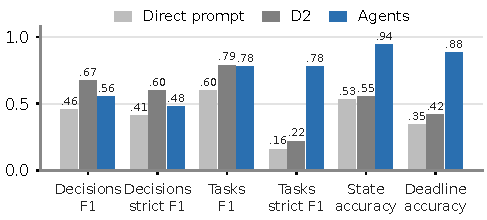
\includegraphics[width=\linewidth]{figures/overview.pdf}

{\tabfont
\begin{tabularx}{\linewidth}{@{}Y rrrrrrr@{}}
\toprule
Condition & dec.\,F1 & tasks F1 & strict D & strict T & state & deadl. & time (s) \\
\midrule
Direct prompt & .458 & .598 & .410 & .161 & .533 & .346 & 180 \\
D2 & \textbf{.673} & .789 & \textbf{.596} & .220 & .551 & .419 & 250 \\
\textbf{Agents (full)} & .556 & .775 & .481 & .775 & .945 & .884 & 1358 \\
\quad $-$ ReAct & .525 & .724 & .424 & .724 & .918 & .833 & 1316 \\
\quad $-$ Auditor & .552 & \textbf{.800} & .476 & \textbf{.800} & .945 & .909 & 484 \\
\quad $-$ Few-shot & .583 & .710 & .450 & .710 & .890 & .868 & 1646 \\
\quad $-$ CoT & .533 & .792 & .450 & .792 & .932 & .929 & 676 \\
\quad $-$ Guards & .488 & .780 & .439 & .780 & .961 & .891 & 1714 \\
\bottomrule
\end{tabularx}
\\[1pt]
{\color{muted} An item matches when its text similarity to the rubric is ${\ge}0.55$ (D2 criterion); strict F1 also requires the right state; state and deadline accuracy are over matched items; time = summed inference per step on a T4.}}

\begin{itemize}
\item \textbf{Tasks, states and deadlines improve a lot:} tasks strict F1 .22$\to$.78 (D2 left 44 tasks \texttt{pending}, the agents none); correct deadlines 42\%$\to$88\%, invented ones 11$\to$3. Per meeting, the agents beat D2 on strict F1 in \textbf{7/10}.
\item \textbf{Decisions regress} (F1 .673$\to$.556): more rejections found (6/11 vs 2/11), fewer pending (1/8 vs 5/8) and conditional ones (2/10 vs 8/10).
\item \textbf{The ablations explain it.} Without the few-shot, decisions F1 rises to .583 and 5/8 pending reappear: the exemplar comes from templated train meetings and pushes terse statements (7 words vs 16 in D2) that the similarity matcher penalizes. The guards are the largest single help for decisions ($-$.068 without them). The Auditor loop costs 2.8$\times$ the time for $\pm$.03.
\item \textbf{Post-hoc check} (replaying the traces, no model calls): dropping the Finalizer's decision/task overlap rule recovers 4 correct decisions but adds 10 wrong ones (.556$\to$.557), so the regression comes from the Decisions agent.
\end{itemize}

\sectionbar{6. FAILURE CASE: M09 (WORST STRICT F1, CRITERION FIXED BEFOREHAND)}
Strict F1 .50, decisions F1 .33 (trace \texttt{runs/test/traces/full/M09.jsonl}). The chain ``Friday $\to$ Monday 16'' collapsed into one \texttt{final} at u16. Tasks turned u17 (``Queda fijada la primera prueba'') into a task, so the Finalizer dropped the correct decision on that turn. Turns that repeat a commitment (u09/u10, u12) became duplicate tasks, and the pending ``future activation'' (u30) was merged into a conditional decision. The Decisions agent is where the next iteration should go: longer statements and one chain per topic.
\par
\sectionbar{7. REPRODUCIBILITY}
The graph is a LangGraph \texttt{StateGraph}; every agent uses Ministral~3B Instruct \texttt{q4\_K\_M} (digest \texttt{f04aa1c7}) on Ollama 0.40.11, temperature 0, seed 42. Each prompt is a versioned file in \texttt{deliverable3/prompts/} with a CHANGELOG. Traces of every input are in \texttt{runs/test/traces/}; the video shows M01. In the Colab notebook, \texttt{MODE='DEMO'} reproduces the video and \texttt{'FULL'} the table.
\end{minipage}

\end{document}
